\documentclass[a4paper,oneside,12pt]{report}
\usepackage{styles/fbe_tez}
\usepackage[utf8x]{inputenc} % To use Unicode (e.g. Turkish) characters
\usepackage{amsmath, amsthm} % Some extra symbols
\usepackage[bottom]{footmisc}
\usepackage{cite}
\usepackage{graphicx}
\usepackage{longtable}
\usepackage{float}
\usepackage{multirow}
\usepackage{subfigure}
\usepackage{algorithm}
\usepackage{algorithmic}
\usepackage{array}
\usepackage{amssymb,bm,cite,graphicx, fixmath, texdraw}
\usepackage{epsfig}
\usepackage{epstopdf}
\usepackage{subfigure} % 
\usepackage{amsmath}
\usepackage{notoccite}

\interdisplaylinepenalty=2500
\hyphenation{lists} \makeatletter

\newcommand{\field}[1]{\mathbb{#1} }
\newcommand{\beq}{\begin{equation} \setlength\abovedisplayskip{5pt} 
\setlength\belowdisplayskip{5pt}}
\newcommand{\eeq}{\end{equation}}
\newcommand{\bea}{\begin{eqnarray}}
\newcommand{\eea}{\end{eqnarray}}
\newcommand{\defn}{\stackrel{\triangle}{=}}
\newcommand{\nn}{\nonumber}
\newcommand{\nnl}{\nonumber \\}
\renewcommand{\theequation}{\arabic{equation}}
\renewcommand{\labelenumi}{(\roman{enumi})}

\DeclareMathOperator*{\argmin}{arg\,min}
\DeclareMathOperator*{\argmax}{arg\,max}

\def\ifundefined{\@ifundefined}
\def\bfat{\left[ \begin{array}}
\def\emat{\end{array} \right]}
\def\bfatt{\left\{ \begin{array}}
\def\ematt{\end{array} \right.}
\def\bset{\left\{ \begin{array}}
\def\eset{\end{array} \right\}}
\def\bpar{\left( \begin{array}}
\def\epar{\end{array} \right)}

\graphicspath{{figures/}} % Graphics will be here

\newtheorem{thm}{Theorem}[chapter]
\newtheorem{prop}[thm]{Proposition}
\newtheorem{lem}[thm]{Lemma}
\newtheorem{cor}[thm]{Corollary}

\numberwithin{equation}{chapter}

% COVER PAGE
\title{THESIS TITLE}
\turkcebaslik{TEZ BAŞLIĞI}
\degree{B.S., Program Name, Boğaziçi University, 2010\\
	M.S., Program Name, Boğaziçi University, 2013}
\author{Name Surname}
\program{Program Name}
\subyear{2019}

% APPROVED BY PAGE
\supervisor{Prof. Name Surname}
%\cosuperi{Title and Name of Cosupervisor I}
%\cosuperii{Title and Name of Cosupervisor II}
\examineri{Assoc. Prof. Name Surname}
\examinerii{Assist. Prof. Name Surname}
\examineriii{Name Surname, Ph.D.}
%\examineriv{}
%\examinerv{}
\dateofapproval{DD.MM.YYYY}

% BEGIN OF DOCS
\begin{document}
\pagenumbering{roman}
\makemstitle % M.S. thesis
\makeapprovalpage

% ACK PAGE
\begin{acknowledgements}
Acknowledgements come here...
\end{acknowledgements}

% ABS PAGE
\begin{abstract}
One page abstract will come here.  
\end{abstract}

% OZET PAGE
\begin{ozet}
Bir sayfa uzunluğunda özet gelecektir.
\end{ozet}

% CONTENTS AND LIST OF FIG AND TABLE PAGES
\tableofcontents
\listoffigures
\listoftables

% LIST OF SYMBOLS PAGE
\begin{symbols}
% The title will be typeset as "LIST OF SYMBOLS".
% Use a separate \sym command for each symbols definition.
% First, Latin symbols in alphabetical order
\sym{$a_{ij}$}{Description of $a_{ij}$}
\sym{$\mathbf{A}$}{State transition matrix of a hidden Markov model}
% 1 EMPTY LINE BETWEEN LATIN AND GREEK SYMBOLS GROUP!!!
\sym{}{}
% Then Greek symbols in alphabetical order
\sym{$\alpha$}{Blending parameter \textit{or} scale}
\sym{$\beta_t(i)$}{Backward variable}
\sym{$\Theta$}{Parameter set}
\sym{ }{}
\end{symbols}

% LIST OF ABBREV PAGE
\begin{abbreviations}
 % Abbreviations in alphabetical order
\sym{2D}{Two Dimensional}
\sym{3D}{Three Dimensional}
\sym{AAM}{Active Appearance Model}
\sym{ASM}{Active Shape Model}
\end{abbreviations}



\chapter{INTRODUCTION}
\label{chapter:introduction}
\pagenumbering{arabic}

The requirements and explanations presented in the following pages aim to
provide guidance to graduate students preparing theses to be submitted to the Institute for
Graduate Studies in Science and Engineering at Bo\u{g}azi\c{c}i
University (henceforth referred to as `the Institute'). These guidelines are not intended, however, as a
complete manual for the writing of theses.

Every thesis must comply with grammatical and formatting rules and must possess clarity of expression. The responsibility for such compliance and
clarity rests primarily upon the candidate; nevertheless, every thesis should be scrutinized for these qualities by the student's Thesis Supervisor and the Defense Jury.


\begin{verbatim}
    vector3d RFField::actOn(Electron2D& e){
        vector3d Efield = getField(e.pos);                            // Calculate E vector
        vector3d F_m = Efield*1E6*eQMratio;                           // Calculate F/m vector
        vector3d acc = (F_m - e.vel*(e.vel*F_m)/(c*c))/e.gamma();     // Calculate a vector
        return acc;
    }
\end{verbatim}


\chapter{FORMAT}
\label{chapter:format}

\section{Character Fonts}

Text should be typed in Times, Times New Roman or Computer Modern
(standard serif font provided by \LaTeX). The font size must be 12 points in the text including formulas, equations, Table headings, Table and Figure captions. Text appearing in Figures and Tables, as well as the text used in superscripts or subscripts, should be at least 8 points. Footnotes, long biographical quotes and extensive quotations should be 10 points.


\section{Spacing}

Spacing of the text material should be 1.5 or, when necessary, integer multiples thereof. The following are exceptions:
\begin{itemize}
 \item Footnotes: single spacing
 \item Long biographical quotes: single spacing
 \item Extensive quotations: single spacing and indented 1 cm relative to the text material.
 \item Equations and equation arrays: single spacing before and after,
 \item Footnotes: single spacing,
 \item Long biographical quotes: single spacing,
 \item Extensive quotations: single spacing and indented 1 cm relative to the text ma-
terial.
\end{itemize}

\clearpage
Spacing of figures is given in the ordered list below:
\begin{enumerate}
 \item Last line of a paragraph,
 \item One line of empty space,
 \item Figure,
 \item One line of empty space,
 \item Figure Caption ,
 \item One line of empty space,
 \item First line of a new paragraph.
\end{enumerate}

Spacing of tables is given in the ordered list below:
\begin{enumerate}
 \item Last line of a paragraph,
 \item One line of empty space,
 \item Table caption,
 \item Half a line of empty space,
 \item Table,
 \item One line of empty space,
 \item First line of a new paragraph.
\end{enumerate}

These spacing may be handed automatically by latex, but not always guaranteed. You should also check manually your thesis for this spacing order

\section{Centering}
\label{sec:centering}

The center point of titles and headings should be 112 mm from the left
edge of the paper or 98 mm from the right edge. This can be accomplished
via the standard centering commands in editors such as Microsoft Word and \LaTeX after margins are set as per explained in the following section. Centering manually is \emph{not} recommended practice because it is prone to errors.


\section{Margins}

Margins of pages should conform to the following specifications:
\begin{itemize}
 \item Left margin: 3.5 cm from the left edge of the paper
 \item Right margin: 2 cm from the right edge of the paper
 \item Top margin: 3.5 cm from the top edge of the paper (page numbers must be 2 cm from the top edge of the paper)
 \item Bottom margin: (at least) 2 cm from the bottom edge of the paper
\end{itemize}

Figures and Tables should also adhere to these margins. Folded pages will not be accepted unless there is absolutely no other way for the material to be presented.


\section{Pagination}

Each page in the thesis should bear a page number except for the title page and the pages on which a Figure or a Table is placed in landscape orientation. Only one side of the paper should be used.

The preliminary section comprising the Title Page, Page of Approval, Dedication Page (if present), Acknowledgements Page (if present) and the other pages in Table \ref{table:pagination} should be numbered, using lower case Roman numerals (i.e. i, ii, iii, ...). The Title Page counts as page i but the page number is not printed.  The preliminary section must follow the sequence shown in Table \ref{table:pagination}. An example of this sequence is provided in Appendix A.

\begin{table}[H]
\centering
\caption{Pagination Table: Page numbers are given as an example where each part takes only one page.}
\vskip\baselineskip
\begin{tabular}{|c|c|}
\hline
 \textbf{Page Title}& \textbf{Number}\\\hline
(Title Page) & Page i (number does not appear) \\\hline
(Page of Approval)  & Page ii \\\hline
(Dedication) & Page iii (if present) \\\hline
ACKNOWLEDGEMENTS & Page iv (if present)\\\hline
ABSTRACT  & Page v \\\hline
ÖZET  & Page vi \\\hline
TABLE OF CONTENTS  & Page vii \\\hline
LIST OF FIGURES  & Page viii (if present) \\\hline
LIST OF TABLES  & Page ix (if present) \\\hline
LIST OF SYMBOLS & Page x (if present) \\\hline
LIST OF ACRONYMS/ABBREVIATIONS & Page xi (if present) \\\hline
\end{tabular}
\label{table:pagination}
\end{table}

For the remainder of the thesis, Arabic numerals should be used. Each page should be numbered unless there is a full-page landscape Figure or Table present on a page; page numbers are not printed on such pages, but the
numbers continue to increment. Page numbers should to be placed two centimeters from the top and the right edges of the pages and they should be in 12 points. Use of suffixes (such as 25a, 25b, etc.) or punctuation (such as a dash or a period) is not permitted in page numbers. The numbering in the main body of the thesis should begin with page 1 and run consecutively to the last page.


\section{Headings}

Headings should be in the same font as the rest of the text and should feature no quotation nor punctuation marks other than the period following the Heading number. There may be at most four levels of Headings: Main Headings, Second Headings, First Subheadings and Second Subheadings. Additionally, special captions to designate Theorems, Corollaries, Lemmas, Definitions, Remarks and Propositions may be deployed.

Headings should be followed by at least one line of text (i.e. Headings should not directly be followed by Tables or Figures).

\begin{table}[H]
    \centering
    \vskip\baselineskip
    \caption{Summary of Heading specifications.}
    \vskip\baselineskip
    \begin{tabular}{|c|c|c|c|c|m{2cm}|}
  \hline
  Main Headings & centered & capital letters & bold face & 14 pt & no period\newline at the end \\
  \hline
  Second Headings & centered & title case letters & bold face & 12 pt & no period\newline at the end \\
  \hline
\end{tabular}
\end{table}


\subsection{Main Headings}

Main Headings should be numbered as 1., 2., ..., and they should comply with the following rules:
\begin{itemize}
 \item Main Headings should begin a new page and should be centered according to
Section \ref{sec:centering}. They should be typed in bold face and should be in capital letters and in
14 points. There should be no period at the end of the heading text.
\item Main Headings should reflect the content of the text that follows.
Main Headings are not to be called as chapters.
\item Heading number should be followed by a period and two spaces.
\item Main Headings should be separated from the succeeding text or second heading by two empty lines of text.
\end{itemize}


\subsection{Second Headings}

Second Headings should be numbered as 2.1., 2.2., ..., and they should comply with the following rules:
\begin{itemize}
 \item Second Headings should be centered according to Section \ref{sec:centering} and be typed in 12 points, bold face and title case letters (i.e., the first letter of each word except conjunctions, prepositions and articles must be a capitalized). There should be no period at the end of the heading text.
\item Heading number should be followed by a period and two spaces.
\item Second headings should be separated from the preceding text or main heading and succeeding text or first subheading by two empty lines of text.
\end{itemize}


\subsection{First Subheadings}

First Subheadings should be numbered as 2.1.1., 2.1.2., ..., and they should comply with the following rules:

\begin{itemize}
\item First Subheadings should be typed in bold face in 12 points and with title
case letters, beginning at the left
margin of the text. There should be no period at the end of the heading text.
%\item There should be no leading text on the line of the first heading.
\item Heading number should be followed by a period and two spaces.
\item First Subheadings should be separated from the preceding text or second heading and succeeding text by one empty line of text.
\end{itemize}


\subsection{Second Subheadings}

Second Subheadings should be avoided if possible. If they can't be avoided, they should be numbered as 2.1.1.1., 2.1.1.2., ..., and they should comply with the following rules:
\begin{itemize}
\item Second Subheadings should be aligned with the left margin of the text (with no indent), should be typed in 12 points and in title case letters, and they should be underlined.
\item Heading number should be followed by a period and
two spaces.
\item Heading text should be followed by a period and the leading text.
\item Second Subheadings should be separated from the preceding text or First Subheading by an empty line of text.
\end{itemize}


\subsection {Special Captions}

Special captions may be deployed to initiate Theorems, Lemmas, Propositions, Corollaries and Definitions. Special captions should obey the following rules:
\begin{itemize}
\item Special captions should be bold and in 12 points, typed in title case letters.
\item Special captions should be on the same line as their leading text, and they should be aligned with the left text margin (with no indent).
\item Leading text appearing after a special caption should be in italics and not more than one paragraph.
\item Each special caption should be succeeded with a numbering label in the form X.Y, where the first number X indicates the number of the current main heading and the second number Y starts with unity for each main heading and increases sequentially and separately for each caption type. For example, 3.5 would mean the fifth special caption of a certain type appearing under the third main heading (e.g. Theorem 3.5). When the main heading pertains to an Appendix, the first indicator is a letter such as A, B, ... .
\item For Theorems, Lemmas and Corollaries, a series of proof or remark blocks may follow. The first proof block should begin with the word \textit{Proof} written in italics and followed by a period; the remaining text of the block and the following blocks are regular type. The last block in a Proof environment should terminate with a $\Box$ at the lower right corner.
\end{itemize}


\section{Paragraphs}

First lines of all paragraphs should be indented by one centimeter. A new paragraph should not begin at the bottom of a page unless \textit{at least two lines} of the paragraph may be printed on that page. Each paragraph should be separated from the preceding and succeeding paragraphs by an empty line of text.


\section{List Items}
Lists composed of successive lines of text or paragraphs may, for clarity, be preceded by a bullet ($\bullet$) or enumerated as (i), (ii), (iii), etc.

Bold face or italic characters should not be used in list items. Certain information such as enzyme lists and lists of chemical supplies should be presented in tables rather than paragraph lists.

Second level of list items are permitted and they must be preceded by a bullet if the first level items are enumerated; on the other hand, if the first level items are preceded by a bullet, then the second level items must be enumerated.

Third level list items are not allowed.


\section{Footnotes}

Footnotes should be avoided whenever possible. If and when they must be used, they should comply with the following rules.
\begin{itemize}
\item Footnote references should be indicated in the text by a superscript Arabic number immediately following the word, phrase or sentence which the footnote concerns.
\item Footnotes should be sequentially numbered on each page and in the entire thesis.
\item Footnotes should be placed at the bottom of the page on which they are indicated. They should be indented from the left margin of the text by one centimeter and should be separated from the main text by a short horizontal line. Footnotes should be single-spaced and 10 points.
\end{itemize}


\section{Bibliographical Material}

The references are listed in the bibliography in the order of appearance in the text and they are numbered accordingly using Arabic numerals as 1., 2. ... (this will be referred to as the ``enumerated reference list"). The numerical reference of bibliographical material should be indicated in the text by an Arabic numeral in square brackets (for example ``[8]") placed in the text immediately following the name, word, phrase, or sentence
which the reference concerns (in some cases, this may be the author's
name). When two bibliographical references are to be cited, they should be separated by a comma (for example ``[8,9]"); when three or more consecutive
bibliographical references are to be cited, the first and the last should be given, separated by a dash line (for example ``[8-12]", ``[6], [8-12], [17]").

In the References section, references which do not exceed 10 authors must be written openly. "et al." expression can only be used when there are more than 10 authors for a reference.


\subsection{Enumerated Reference Lists}

The following schemes should be used in the enumerated reference lists: 

\begin{flushleft}

\leftskip 5mm \parindent -5mm \textbf{Books:}

\leftskip 5mm \parindent -5mm 1. Firstauthorsurname, F.A. and S.A. Surname, \textit{Title of the Book}, Second Edition (only if other than the first), Publisher Name, City, Year.

\leftskip 5mm \parindent -5mm 2. Ross, S., \textit{A First Course in Probability}, Seventh Edition, Pearson Prentice Hall, New Jersey, 2006.

\leftskip 5mm \parindent -5mm 3. Ang, A.H-S. and W.H. Tang, \textit{Probability Concepts in Engineering}, John Wiley \& Sons, New Jersey, 2007.

\leftskip 5mm \parindent -5mm 4. Ang, A.H-S., W.H. Tang and S. Ross, \textit{Probability Concepts in Engineering}, John Wiley \& Sons, New Jersey, 2007.\newline


\leftskip 5mm \parindent -5mm \textbf{Journal Articles:}

\leftskip 5mm \parindent -5mm 1. Firstauthorsurname, F.A. and S.A. Surname, ``Title of the Article", \textit{Title of the Journal}, Vol. X, No. Y, page number (p. 5 or pp. 5-10), year of publication.

\leftskip 5mm \parindent -5mm 2. Maiers, J. and Y.S. Sherif, ``Application of Fuzzy Set Theory", \textit{IEEE Transactions on Systems, Man, and Cybernatics}, Vol. 15, No. 1, pp. 41-48, 1985.\newline


\leftskip 5mm \parindent -5mm \textbf{Conference Proceedings:}

\leftskip 5mm \parindent -5mm 1. Firstauthorsurname, F.A. and S.A. Surname, ``Title of the Article", in \textit{Title of the Proceedings}, Editors, Location, Vol. X (if exists), page number (p. 5 or pp. 5-10), year.

\leftskip 5mm \parindent -5mm 2. Brown, D. and D. Clair, ``Integrated R-transportation", paper presented at the \textit{14th International Conference of Transportation Logistics}, Istanbul, Turkey, 2008.\newline

\clearpage
\leftskip 5mm \parindent -5mm \textbf{Dissertations:}

\leftskip 5mm \parindent -5mm 1. Authorsurname, F.A., \textit{Title of the Dissertation}, Level (Ph.D. Thesis or M.S. Thesis), Name of Higher Education Institute, Year.

\leftskip 5mm \parindent -5mm 2. İşgüder, E., \textit{Human Computer Interaction in the 21st Century}, M.S. Thesis, Boğaziçi University, 2015.

\leftskip 5mm \parindent -5mm 3. İşgüder, E., \textit{Human Computer Interaction in the 22st Century}, Ph.D. Thesis, Boğaziçi University, 2021.\newline


\leftskip 5mm \parindent -5mm \textbf{Websites:}

\leftskip 5mm \parindent -5mm 1. Authorsurname, F.A. AND/OR Name of Authoring Body/Organization, ``Title of the Web Material", Publishing Year, URL, last access date.

\leftskip 5mm \parindent -5mm 2. Sarp, B., ``Observations", 2001, http://sarp.com.tr/obs.html, accessed on November 21, 2015.

\leftskip 5mm \parindent -5mm 3. Wikipedia, ``John von Neumann", http://en.wikipedia.org/wiki/John\_von\_Neumann, accessed on October 30, 2015.

\leftskip 5mm \parindent -5mm 4. Wikipedia, http://en.wikipedia.org/, accessed on October 29, 2015.

\leftskip 5mm \parindent -5mm 5. http://encyclopedia.org/, accessed on October 21, 2015.\newline

\clearpage
\leftskip 5mm \parindent -5mm \textbf{Patents:}

\leftskip 5mm \parindent -5mm 1. Lastname F., "Title of Patent", U.S. Patent Number, Month Day, Year. Available: URL or Database Name, Accessed on: Month Day, Year.

\leftskip 5mm \parindent -5mm 2. Shatner W., L. a. Christel, D. A. Borkholder and S. J. Young, ``Apparatus for Analysis of a Nucleic Acid Amplification Reaction", U.S. Patent 6942971 B2, September 13, 2005. https://www.google.com/patents/US6942971, Accessed on December 12, 2017.\newline


\leftskip 5mm \parindent -5mm \textbf{Manuals:}

\leftskip 5mm \parindent -5mm 1. Name of Manual/Handbook, xth ed. Name of Comp.,  Country, Month. Year, pp. xxx-xxx (pages if relevant). Accessed on: Month, Day, Year. [Online].site/path/file 

\leftskip 5mm \parindent -5mm 2. The MakerBot Replicator Desktop 3D Printer (Fifth Generation Model) User Manual, MakerBot Industries, Brooklyn, NY, 2014.\newline


\leftskip 5mm \parindent -5mm \textbf{Preprints:}

\leftskip 5mm \parindent -5mm 1. Authorsurname, F.A., ``Title of the 
Material", arxiv Preprint number, Publishing Year.

\leftskip 5mm \parindent -5mm 2. Nettelblahd J. and C. Nettelblahd, “CannyFS: Opportunistically Maximizing I/O Throughput Exploiting the Transactional Nature of Batch-Mode Data Processing”, arXiv:1612.06830 [cs], 2016.\newline
\end{flushleft}

\subsection{Surname Reference Lists}

The following schemes should be used in the surname reference lists:\newline


\leftskip 5mm \parindent -5mm \textbf{Books:}

\leftskip 5mm \parindent -5mm Firstauthorsurname, F.A. and S.A. Surname, Year \textit{Title of the Book}, Second Edition (only if other than the first), Publisher Name, City.

\leftskip 5mm \parindent -5mm Ross, S., 2006, \textit{A First Course in Probability}, Seventh Edition, Pearson Prentice Hall, New Jersey.

\leftskip 5mm \parindent -5mm Ang, A.H-S. and W.H. Tang, 2007, \textit{Probability Concepts in Engineering}, John Wiley \& Sons, New Jersey.

\leftskip 5mm \parindent -5mm Ang, A.H-S., W.H. Tang and S. Ross, 2007, \textit{Probability Concepts in Engineering}, John Wiley \& Sons, New Jersey.\newline


\leftskip 5mm \parindent -5mm \textbf{Journal Articles:}

\leftskip 5mm \parindent -5mm Firstauthorsurname, F.A. and S.A. Surname, year of publication, ``Title of the Article", \textit{Title of the Journal}, Vol. X, No. Y, page number (p. 5 or pp. 5-10).

\leftskip 5mm \parindent -5mm Maiers, J. and Y.S. Sherif, 1985, ``Application of Fuzzy Set Theory", \textit{IEEE Transactions on Systems, Man, and Cybernatics}, Vol. 15, No. 1, pp. 41-48.\newline

\clearpage
\leftskip 5mm \parindent -5mm \textbf{Conference Proceedings:}

\leftskip 5mm \parindent -5mm Firstauthorsurname, F.A. and S.A. Surname, year, ``Title of the Article", in \textit{Title of the Proceedings}, Editors, Location, Vol. X (if exists), page number (p. 5 or pp. 5-10).

\leftskip 5mm \parindent -5mm Brown, D. and D. Clair, 2008, ``Integrated R-transportation", paper presented at the \textit{14th International Conference of Transportation Logistics}, Istanbul, Turkey.\newline 


\leftskip 5mm \parindent -5mm \textbf{Dissertations:}

\leftskip 5mm \parindent -5mm Authorsurname, F.A., Year, \textit{Title of the Dissertation}, Level (Ph.D. Thesis or M.S. Thesis), Name of Higher Education Institute, Year.

\leftskip 5mm \parindent -5mm İşgüder, E., 2015, \textit{Human Computer Interaction in the 21st Century}, M.S. Thesis, Boğaziçi University.

\leftskip 5mm \parindent -5mm İşgüder, E., 2021, \textit{Human Computer Interaction in the 22st Century}, Ph.D. Thesis, Boğaziçi University.\newline


\leftskip 5mm \parindent -5mm \textbf{Websites:}

\leftskip 5mm \parindent -5mm Authorsurname, F.A. AND/OR Name of Authoring Body/Organization, Publishing Year, ``Title of the Web Material", URL, last access date.

\leftskip 5mm \parindent -5mm Sarp, B., 2001, ``Observations", http://sarp.com.tr/obs.html, accessed on November 21, 2015.

\clearpage
\leftskip 5mm \parindent -5mm Wikipedia, ``John von Neumann", http://en.wikipedia.org/wiki/John\_von\_Neumann, accessed on October 30, 2015.

\leftskip 5mm \parindent -5mm Wikipedia, http://en.wikipedia.org/, accessed on October 29, 2015.

\leftskip 5mm \parindent -5mm http://encyclopedia.org/, accessed on October 21, 2015.\newline


\leftskip 5mm \parindent -5mm \textbf{Patents:}

\leftskip 5mm \parindent -5mm Lastname F., Year, "Title of Patent", U.S. Patent Number. Available: URL or Database Name, Accessed on: Month Day, Year.

\leftskip 5mm \parindent -5mm Shatner W., L. a. Christel, D. A. Borkholder and S. J. Young, 2005, ``Apparatus for Analysis of a Nucleic Acid Amplification Reaction", U.S. Patent 6942971 B2, September 13, 2005. https://www.google.com/patents/US6942971, Accessed on December 12, 2017.


\leftskip 5mm \parindent -5mm \textbf{Manuals:}

\leftskip 5mm \parindent -5mm Name of Manual/Handbook, Year, xth ed. Name of Comp.,  Country, pp. xxx-xxx (pages if relevant). Accessed on: Month, Day, Year. [Online].site/path/file 

\leftskip 5mm \parindent -5mm The MakerBot Replicator Desktop 3D Printer (Fifth Generation Model) User Manual, 2014, MakerBot Industries, Brooklyn, NY.\newline


\leftskip 5mm \parindent -5mm \textbf{Preprints:}

\leftskip 5mm \parindent -5mm Authorsurname, F.A., Publishing Year, ``Title of the 
Material", arXiv Preprint number.

\leftskip 5mm \parindent -5mm Nettelblahd J. and C. Nettelblahd, 2016, “CannyFS: Opportunistically Maximizing I/O Throughput Exploiting the Transactional Nature of Batch-Mode Data Processing”, arXiv:1612.06830 [cs].

\leftskip -5mm
\parindent 10mm

\section{Mathematical Expressions}
Mathematical expressions such as equations, formulas, etc. should be typeset in accordance with the following rules:

\begin{itemize}
\item Mathematical symbols and expressions within the text should be written with the same font used in the equation or equation array environments in order to separate them from the regular text. Italic font is the typical choice. \\

\item  Mathematical expressions, equations and equation arrays should be part of the text and should not be treated as images or floating objects. This means that i) they should be placed with one line spacing between the preceding and following text, ii) if they finish the sentence they should be ended with a full stop (.), iii) if the sentence continues after the mathematical expression it should not have a paragraph indentation or it should not start with a capital letter. \\

\item Multiple equations or mathematical expressions should be written in an equation array environment. This guarantees the single line spacing between these expressions. In equation arrays, the individual lines should be aligned such that the first equality (or inequality or similarity) signs are in line with each other.\\

\item Mathematical expressions should be referred to after they appear first and not before. Try to avoid from forward referencing. \\

This equation template should be followed strictly. You can see detailed examples in the Examples section.

\end{itemize}

\section{Tables and Figures}

All floating items such as graphs,
charts, photographs, illustrations and lists should be considered and
designated as a Figure or a Table, whichever is appropriate. To ensure acceptable print, all drawings, graphs, illustrations and similar graphical material should be prepared with sufficient resolution. All text in Figures and Tables should be clearly legible with and should appear in at least 8 points.

All Tables and Figures should be captioned and enumerated in the form ``X.Y" wherein ``X" refers to the number (or letter, if in Appendix) of the current Main Heading, and ``Y" increases sequentially staring with unity at each Main Heading, separately for Figures and Tables. Table captions should be located above the Tables whereas Figure captions should be placed below the Figures.  All captions should include the label and the number followed by a period and a space (such as ``Table 3.1. " or ``Figure A.1. " if in appendix), followed by an explanatory text referring to the content of the Table or Figure. Only the first word of the caption text should be capitalized and the text should end with a period; it should not be boldface or italic.

All Figures, Tables and their captions should be centered in accordance with Section \ref{sec:centering}. Captions should continue at most for 5 lines. Further explanation should be provided in the main text. Reference to a Figure/Table may come before or after the Figure/Table as long as the reference is clearly indicated and understood. If there are too many consecutive and related Figures/Tables, they should be presented in the appendix.

When a Figure contains sub-figures, each sub-figure must be marked with a lowercase letter in parenthesis starting with ``(a)". There is to be a single caption for the whole Figure within which each sub-figure is explicitly referred to and explained (such as ``Figure 3.8. (a) The picture, (b) the bigger picture.").

Figures should not be divided to and continued on multiple pages. When a Table is divided into two or more pages, each part should have the same label, number and text in its caption, but the captions of the second and the latter parts should end with the expression ``(cont.)." to indicate continuation.

When a Table or a Figure is referenced in the text, the reference should include the label and the number with the first letter of the label in capital case (such as
``Table 4.5" or ``Figure 3.8" - note that no period is placed after the number). A sub-figure may be directly referenced by indicating its label, number and sequence (such as ``Figure 3.8a" or ``Figure 3.8a and c").

All Tables should be framed, both externally and internally, with single-line borders. Tables should not have any background color, and the text fonts used in the Tables should
be consistent with the rest of the text. Table headers may be boldface
but colored texts are not allowed in these headers. Figures may be
colored where necessary. Figures should not have an embedded title in
the graphics/charts/photographs/etc., and the Figure caption should include all the necessary information.

All axes of graphs should have titles.



\chapter{ARRANGEMENT}



\section{Title Page}
The Title Page is the first page of the thesis. Please refer to the example for all pertinent details, including proper scaling and positioning. In particular,
\begin{itemize}
\item Page number should not be printed on the Title Page (whose page number is i).
\item The title of the thesis should be centered and in all capital letters in 14 points.
\item All prior higher education degrees of the candidate should be listed on the Title Page, showing the majors, the degree granting institutions and
graduation years in chronological order.
\item The submission requirement (``[...] of the requirements for the degree of Master of Science" or ``[...] of the requirements for the degree of Doctor of Philosophy") should be specified.
\item The name of the graduate program enrolled to and the year in which the thesis is approved should appear at the bottom of the Title Page.
\end{itemize}


\section{Approval Page}
All copies of the submitted thesis should include original signatures
of the Defense Jury on the Approval Page. The Approval Page should appear right after the Title Page.

The names of the members of the Defense Jury
should be listed in the alphabetical order of their surnames except for the
Thesis Supervisor's, whose name should be the first one on the list. If a Co-Supervisor exists, her/his name should appear right after the Supervisor's.
Titles of the Jury members should be presented in the North American
style with either ``Prof.",  ``Assoc. Prof." or ``Assist. Prof." preceding a Jury
member's name. If desired and appropriate, the term `Ph.D.' may follow
a Jury member's name (separated by a comma from the name). Space for the
signature of each Jury member should be left beside each name. 

The date at the bottom of the Approval Page is the date at which the thesis is
approved by the Defense Jury.


\section{Dedication}
Dedication is rare and it should be thought of as an honorific statement to explicitly recognize someone who has provided exceptional support to the author, especially in the completion of the thesis. The Dedication Page should come right after the Approval Page.
Dedications should be simple phrases (such as `To my mother."), in English, and placed at the lower right corner of the page.


\section{Acknowledgements}
The candidate may desire to include a page with a brief note of an
acknowledgement of help received from particular people in the preparation of the thesis. All organizations proving financial support must be acknowledged and
grant numbers should be included. 

\section{Abstract}
The Abstract should briefly describe the thesis work including its objectives, methods, results and conclusions. Two abstracts, one in
English and the other in Turkish, should be included. The Abstract
should not contain headings, tabular material, chemical formulae, footnotes or references, but author citing is allowed. Each abstract should be at most one page long. 

The Abstract Page should contain the title of the thesis. The Turkish Abstract (``\"{O}zet") must follow the English Abstract in the same format.


\section{Table of Contents, List of Figures, List of
Tables, List
of Symbols and List of Acronyms/Abbreviations}
Theses are expected to have a `Table of Contents' for the convenience
of the reader. The Table of Contents should not list itself.

If Figures and Tables are scattered throughout the text, a
separate `List of Figures' (and/or `List of Tables') must be included
after the Table of Contents. These lists should include page numbers.

Similarly, a `List of Symbols' and/or `List of Symbols/Abbreviations', whichever is
appropriate, should be included. `List of Symbols' should list symbols alphabetically as separate groups in the order of Latin symbols, Greek symbols, and other symbols. `List of Accronyms/Abbreviations' should contain abbreviations listed alphabetically.

\section{The Main Body of the Thesis}
The main body of the thesis begins with the first Main Heading. The main body
should be composed of a series of Main Headings, starting with an
`Introduction' and ending with a `Conclusion'. The
main body generally includes one or more of the following: `Literature Survey', `Problem Statement', `Materials and Methods', `Results and Discussions' or other relevant topics.

The first page of the first Main Heading should be the first page
enumerated in Arabic numerals. 

Attention should be paid to the precautions listed below:

\begin{itemize}
\item The whole text should be left and right justified.
\item Please note the spelling of `Foreword'.
\item Periods, commas, semicolons and colons go outside the quotation
marks.
\item The word `data' is plural and requires a plural verb.
\item Integers from one to nine, inclusive, should be spelled out
except when they represent a chapter or a section; for numbers 10 and
above, use numerals. Numbers should be spelled out when they begin a
sentence.
\item Do not spell out per cent; use \%.
\end{itemize}


\section{Appendices}
A thesis may present supporting data in the form of one or more Appendices. Examples of Appendix material include data sheets, questionnaire samples, flowcharts, illustrations, maps,
software listings, charts, etc. If the appended data need to include
oversized illustrations or maps, several alternative methods of
inclusions are available.

If a Table, Figure, Equation etc., is to be included in an
Appendix, the numbering should follow the same rules used within
the main body of the thesis. In this case, however, the numbering should begin with the letter
of the respective Appendix such as ``Table A.1", ``Equation B.4" etc.
Each Appendix should have a descriptive title, as should all Main Headings.

Software/computer programs developed in the thesis should be submitted on a separate CD. The format and contents of this CD is explained in Appendix B.



\chapter{PREPARATION OF THE FINAL COPIES}


\section{Typesetting}
Typesetting is generally accomplished using custom programs such as \TeX{}, \LaTeX{} or Microsoft Word\textsuperscript{\textregistered}. Template files may be provided by the Institute. It is the responsibility of the author to ensure that the typeset manuscript complies with the rules and regulations specified in this guide.


\section{Paper Quality}
The original copy should be printed on 75 or 80 gr/m\textsuperscript{2}, white, A4 paper. All reproduced copies should be of the same grade of paper.


\section{Printer}
The printer used in printing the thesis copies should provide high quality outputs such as laser or ink jet printers. Printer settings should comply with A4 and there should be no resizing of the page in printing.


\section{Reproduction}
Photocopy reproduction is acceptable while mimeographed or ditto
copies are not acceptable for all parts or copies of the thesis
submitted to the Institute or to the Library. Care should be taken to
insure that the proper grade of paper is used at all times and that
copying contrast is dark.


\section{Binding}
The thesis should be bound in dark blue, hard cover. The size of final, bound
copy of the thesis should conform to A4 paper size. The name and surname of
the candidate, the degree obtained and the year should be
printed, in the order specified, on the spine of the cover. When the thesis
is placed front cover up, the spine should read from left to right.



\chapter{PUBLICATION OF THESES}


\section{Use of Copyrighted Material}
The thesis author is solely responsible for use of any
copyrighted material in the thesis. 

Permission to quote extensively from copyrighted material or to
reproduce a figure should be obtained by the thesis author from the author 
or the publisher of the copy righted material, whichever holds the copyright. Customarily,
authorization is granted on the condition that proper acknowledgement
is given. In some instances, however, the thesis author should keep on file the copyright granting permission to address possible future inquiries.


\section{Publications}
Theses or extracts thereof may be published in scholarly journals, proceedings, books or other media only upon release for publication by the major supervisor and provided proper credit is
given to Bo\u{g}azi\c{c}i University. No thesis may be published as
such before it has been approved by the major supervisor. All theses
and separately submitted abstracts are the property of Bo\u{g}azi\c{c}i
University.

As many theses will be important to other scholars and to a more
general body of readers, candidates for degrees should plan for
publication of their work. 




\chapter{EXAMPLES}
\label{chapter:experiments-and-results}

Experiments and results come here... 
\section{Sample Section}
Always place some text after headings before putting a graphics into a section as seen in Figure~\ref{fig:sinAndCosineSample}. 

\begingroup
\vskip\baselineskip % Only use if necessary
\begin{figure}[htbp]
	 \centering
		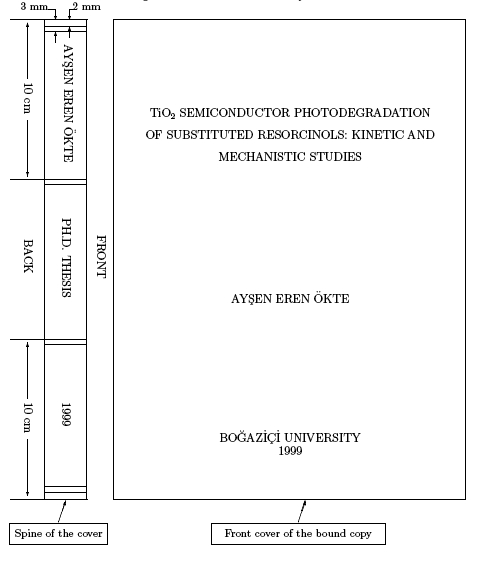
\includegraphics[width=0.5\columnwidth]{figures/cover.jpg}
		\vskip\baselineskip % Leave a vertical skip below the figure
		\caption{FBE Booklet.}
		\label{fig:sinAndCosineSample}
\end{figure}
\endgroup
Also, below, you can find how to arrange figures that can span multiple pages.

Descriptive text explaining the continuation of Figure~\ref{fig:sampleWithContinuation}. Normally FBE expects this page to be fully filled with content, hence the need for shifting text from following pages into here.

\newpage
Now, let us cite some studies: one source as \cite{ArticleRef},  two
sources as \cite{ArticleRef,BookRef} or you may cite three or
more sources as 
\cite{ConferenceRef,Webref,ThesisRef}.
Observe that they are ordered in the references chapter in the same
order as
they are cited. Both the IEEE referencing and APA referencing methods are allowed. 

\begingroup
\begin{figure}[H]
\vskip\baselineskip % Only use if necessary
	\centering
		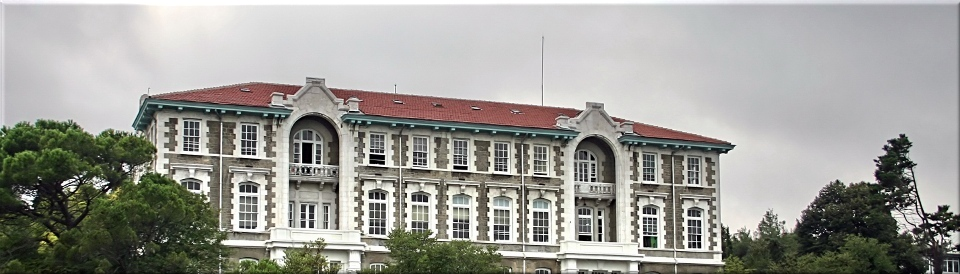
\includegraphics[width=\textwidth, keepaspectratio]{figures/ana-sayfa-cover-03.jpg}
		\caption{Sample Figure.}
		\label{fig:sampleWithContinuation}
		%\vskip\baselineskip 
\end{figure}
\endgroup

\clearpage

\begingroup
\setlength{\belowcaptionskip}{-20pt} %%Only use when there is tto much space below the caption.
\begin{figure}[H]
%\vskip\baselineskip % Only use if necessary
	\centering
		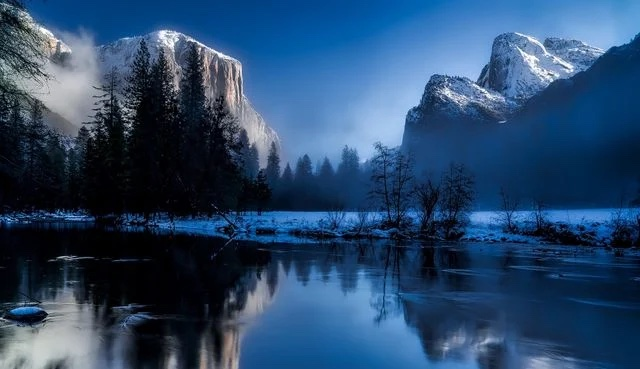
\includegraphics[width=\textwidth, keepaspectratio]{figures/View.jpg}
		\caption{Sample Figure (cont.).}
		\label{fig:sampleWithContinuation2}
\end{figure}
\endgroup

Let us put a sample table as seen in Table~\ref{table:shortTable}. Please pay attention that the caption is followed
by a period.

\begingroup
\begin{table}[thbp]
\vskip\baselineskip 
\caption[Sample table]{Sample table.} %You can also use belowcaptionskip or abovecaptionskip here
\begin{center}
\begin{tabular}{|c|c|c|} \hline
 & \textbf{Header 1}& \textbf{Header 2}\\\hline
\textbf{Row 1} & blah blah blah& blah blah blah \\\hline
\textbf{Row 2} & blah blah blah  & blah blah blah \\\hline
\end{tabular}
\label{table:shortTable}
\end{center}
\end{table}
\endgroup

Next up, there is a sample table that spans multiple pages. Normally the packages that are used for this breaks the formatting package provided by FBE, but if done like this, you won't encounter the ``package conflict" error stated in the FrequentlySeenMistakes.pdf in the FBE web site.
\clearpage

\begingroup
\begin{table}[thbp]
	\caption[Sample table that spans multiple pages.]{Sample table that spans multiple pages.}
	\label{table:multiPageSample}
\end{table}
\begin{center}
	\addtocounter{table}{-1}
	\begin{longtable}{|l|l|}\hline
		\endfirsthead
		\multicolumn{2}{c}{Table \ref{table:multiPageSample}. Sample table that spans multiple pages. (cont.) \vspace{1em}} \\\hline
		\endhead
		\endfoot
		\endlastfoot
		
		\textbf{Header 1}& \textbf{Header 2}\\\hline
		blah blah blah & blah blah blah \\
		& blah blah blah \\
		& blah blah blah \\
		& blah blah blah \\
		& blah blah blah \\
		& blah blah blah \\
		& blah blah blah \\
		& blah blah blah \\
		& blah blah blah \\
		& blah blah blah \\
		& blah blah blah \\\hline
		
		blah blah blah & blah blah blah \\
		& blah blah blah \\
		& blah blah blah \\
		& blah blah blah \\
		& blah blah blah \\
		& blah blah blah \\\hline
		
		blah blah blah & blah blah blah \\
		& blah blah blah \\\hline
		blah blah blah & blah blah blah \\
		& blah blah blah \\
		& blah blah blah \\
		& blah blah blah \\
		& blah blah blah \\
		& blah blah blah \\
		& blah blah blah \\
		& blah blah blah \\\hline
		
		\pagebreak
		\textbf{Header 1}& \textbf{Header 2}\\\hline
		blah blah blah & blah blah blah \\
		& blah blah blah \\
		& blah blah blah \\\hline
		
		blah blah blah & blah blah blah \\
		& blah blah blah \\
		& blah blah blah \\
		& blah blah blah \\\hline
		
		blah blah blah & blah blah blah \\
		& blah blah blah \\
		& blah blah blah \\
		& blah blah blah \\
		& blah blah blah \\\hline
	\end{longtable}
\end{center}
\vskip -2cm %This is used to remove excessive space after the longtable. It's not mandatory, can be removed if the final output isn't as desired.
\endgroup

You can use the code of Table~\ref{table:multiPageSample} to create multiple page spanning longtables.

Footnotes should be avoided as possible. If there is an absolute
necessity, footnotes should be used as this.\footnote{Example of a
footnote}  Please be informed that URLs are not allowed within thesis text, even in footnotes. Provide them as citations instead.

Item lists may be represented as follows:

\begin{itemize}
 \item This is an item. Do not use boldface for the items.
\begin{enumerate}
 \item This is a sub-item. Subsub-items are not allowed.
\end{enumerate}
\item Another item.
\end{itemize}
%  \item 
% \end{enumerate}

Item lists may also be represented as follows:
\begin{enumerate}
 \item This is another enumerated item.
\begin{itemize}
 \item This is another sub-item.
\end{itemize}

\end{enumerate}

{\textbf{Good Equation Example 1:}}

``Notice that the spectral efficiency of the system is $R=n+m=\log_2(NM)$ bits per channel use (bpcu).  At each transmission instant,  each set of $n+m$ bits is split into groups of $n$ and $m$ bits." (Because the letters $N$, $M$, $n$, and $m$ are used to denote some mathematical entities they are written in the math environment.)\\

{\textbf{Good Equation Example 2:}}
The received signal is expressed as
\beq
{\mathbf y}={\mathbf H}{\bf \Psi}{\mathbf x} + {\bm{\nu}} 
\eeq where ${\bf H}$ is the $N_r \times N_t$ dimensional channel matrix and ${\mathbf y}$ and ${\bm{\nu}} $ are the $N_r \times 1$ dimensional received signal and channel noise vectors, respectively. \\

{\textbf{Good Equation Example 3:}}
The received signal is expressed as
\beq
{\mathbf y}={\mathbf H}{\bf \Psi}{\mathbf x} + {\bm{\nu}}. 
\eeq In this expression, ${\bf H}$ is the $N_r \times N_t$ dimensional channel matrix and ${\mathbf y}$ and ${\bm{\nu}} $ are the $N_r \times 1$ dimensional received signal and channel noise vectors, respectively. \\

{\textbf{Good Equation Example 4 (Equation Group):}}
Notice that under the signal model presented in the previous section, ${\mathbf z}$ forms a zero-mean proper complex Gaussian random vector with the mean vector, ${\bf m}_{\bf z}$, that can be written as
\bea{\bf m}_{\bf z} &=& \mbox{E} \left[{\bf z}\right]= \sqrt{\frac{\rho K}{K+1}}\left( \bar{\bf h}_u \psi_u X_v -\bar{\bf h}_{\hat{u}} \psi_{\hat{u}} X_{\hat{v}}\right)\nnl
&=&\sqrt{\frac{\rho K}{K+1}}\left( \bar{\bf h}_u a_u X_v e^{j\theta_u}-\bar{\bf h}_{\hat{u}} a_{\hat{u}} X_{\hat{v}}e^{j\theta_{\hat{u}}}\right)\eea and the covariance matrix,  ${\bf \Sigma}_{\bf z}$, that can be computed as
\beq
{\bf \Sigma}_{\bf z} =\frac{\rho  \gamma(u, \hat{u}, v, \hat{v}, \psi_u, \psi_{\hat{u}}) {\bf \Sigma}_r}{K+1} 
\eeq 
where $\rho$  and ${\bf \Sigma}_r$ are  as defined before.\\

{ \textbf{Good Equation Example 5:} }

The SINR for the users in $\hat{U}_1$, the SNR for the users in $U_2$ on each subcarrier $n$ and the SNR for the remaining users in $\tilde{U}_1$ on each subcarrier $k$ can be written as
\bea
\Gamma^{(n)}_{\hat{U}_1} &=& \frac{P_n |h_n|^2}{P_{N+n} |h_{N+n}|^2 + \sigma^2} = \frac{P_t |g_n|^2}{\epsilon P_t |g_{N+n}|^2 + \sigma^2} \\
\Gamma^{(n)}_{U_2} &=& \frac{P_{N+n} |h_{N+n}|^2}{P_n |a_n - \hat{a}_n|^2 |h_n|^2 + \sigma^2} \nonumber \\
&=& \frac{\epsilon P_t |g_{N+n}|^2}{P_t |a_n - \hat{a}_n|^2 |g_{n}|^2 + \sigma^2}\\
\Gamma^{(k)}_{\tilde{U}_1} &=& \frac{P_{k} |h_{k}|^2}{\sigma^2} = \frac{P_t |g_{k}|^2}{\sigma^2}
\eea
respectively, where $n \in \{1, ..., M\}$, $k \in \{M+1, ..., N\}$. \\


{ \textbf{Bad Equation Example 1:} (Extra space between the text and the mathematical expressions.)}

The received signal is expressed as\

\beq
{\mathbf y}={\mathbf H}{\bf \Psi}{\mathbf x} + {\bm{\nu}} 
\eeq\

 where ${\bf H}$ is the $N_r \times N_t$ dimensional channel matrix and ${\mathbf y}$ and ${\bm{\nu}} $ are the $N_r \times 1$ dimensional received signal and channel noise vectors, respectively. \\
 
{\textbf{ Bad Equation Example 2:} (Paragraph indent and/or capital letter use after an equation despite the fact that the sentence is continued.)}

The received signal is expressed as

\beq
{\mathbf y}={\mathbf H}{\bf \Psi}{\mathbf x} + {\bm{\nu}} 
\eeq

\hspace{.2in} Where ${\bf H}$ is the $N_r \times N_t$ dimensional channel matrix and ${\mathbf y}$ and ${\bm{\nu}} $ are the $N_r \times 1$ dimensional received signal and channel noise vectors, respectively. \\

{ \textbf{Bad Equation Example 3:} (Equation appearing as a floating object instead being attached to a sentence.)}

The received signal is expressed as follows:
\beq
{\mathbf y}={\mathbf H}{\bf \Psi}{\mathbf x} + {\bm{\nu}} 
\eeq In this expression, ${\bf H}$ is the $N_r \times N_t$ dimensional channel matrix and ${\mathbf y}$ and ${\bm{\nu}} $ are the $N_r \times 1$ dimensional received signal and channel noise vectors, respectively. \\


{ \textbf{Bad Equation Example 4:} (Spacing) }

The SINR for the users in $\hat{U}_1$, the SNR for the users in $U_2$ on each subcarrier $n$ and the SNR for the remaining users in $\tilde{U}_1$ on each subcarrier $k$ can be written as\

\beq
\Gamma^{(n)}_{\hat{U}_1} = \frac{P_n |h_n|^2}{P_{N+n} |h_{N+n}|^2 + \sigma^2} = \frac{P_t |g_n|^2}{\epsilon P_t |g_{N+n}|^2 + \sigma^2}\eeq\

\beq \Gamma^{(n)}_{U_2} = \frac{P_{N+n} |h_{N+n}|^2}{P_n |a_n - \hat{a}_n|^2 |h_n|^2 + \sigma^2} = \frac{\epsilon P_t |g_{N+n}|^2}{P_t |a_n - \hat{a}_n|^2 |g_{n}|^2 + \sigma^2} \eeq\

\beq \Gamma^{(k)}_{\tilde{U}_1} = \frac{P_{k} |h_{k}|^2}{\sigma^2} = \frac{P_t |g_{k}|^2}{\sigma^2} \eeq\

respectively, where $n \in \{1, ..., M\}$, $k \in \{M+1, ..., N\}$. \


{ \textbf{Bad Equation Example 5:} (Forward Referencing)}

The received signal is expressed as in Equation (\ref{rec_sig5-}) given below:
\beq
\label{rec_sig5-}
{\mathbf y}={\mathbf H}{\bf \Psi}{\mathbf x} + {\bm{\nu}}. 
\eeq
 ${\bf H}$ is the $N_r \times N_t$ dimensional channel matrix and ${\mathbf y}$ and ${\bm{\nu}} $ are the $N_r \times 1$ dimensional received signal and channel noise vectors, respectively. \\


{ \textbf{Bad Equation Example 6:} }

The received signal is expressed as
\beq
\label{rec_sig6-}
{\mathbf y}={\mathbf H}{\bf \Psi}{\mathbf x} + {\bm{\nu}}.
\eeq
 In Equation (\ref{rec_sig6-}), ${\bf H}$ is the $N_r \times N_t$ dimensional channel matrix and ${\mathbf y}$ and ${\bm{\nu}} $ are the $N_r \times 1$ dimensional received signal and channel noise vectors, respectively.



\chapter{CONCLUSION}
\label{chapter:conclusion}

The conclusions of the thesis should come
here.
% \nocite{NewEntry1,NewEntry2,NewEntry3,NewEntry4,NewEntry5,
% NewEntry6,
% NewEntry7,NewEntry8,NewEntry9,NewEntry10,NewEntry11,NewEntry12}

\nocite{*}
 \bibliographystyle{styles/fbe_tez_v11.bst} %Still may have problems
\bibliography{references} %Still may have problems
 
 
 
\chapter*{REFERENCES FOR APA STYLE}

\leftskip 5mm \parindent -5mm Ang, A.H-S., W.H. Tang and S. Ross, \textit{Probability Concepts in Engineering}, John Wiley \& Sons, New Jersey, 2007.

\leftskip 5mm \parindent -5mm Brown, D. and D. Clair, 2008, ``Integrated R-transportation", paper presented at the \textit{14th International Conference of Transportation Logistics}, Istanbul, Turkey.

\leftskip 5mm \parindent -5mm İşgüder, E., 2021, \textit{Human Computer Interaction in the 22st Century}, Ph.D. Thesis, Boğaziçi University.

\leftskip 5mm \parindent -5mm Maiers, J. and Y.S. Sherif, 1985, ``Application of Fuzzy Set Theory", \textit{IEEE Transactions on Systems, Man, and Cybernatics}, Vol. 15, No. 1, pp. 41-48.

\leftskip 5mm \parindent -5mm Nettelblahd J. and C. Nettelblahd, 2016, “CannyFS: Opportunistically Maximizing I/O Throughput Exploiting the Transactional Nature of Batch-Mode Data Processing”, arXiv:1612.06830 [cs].

\leftskip 5mm \parindent -5mm Sarp, B., 2001, ``Observations", http://sarp.com.tr/obs.html, accessed on November 21, 2015.

\leftskip 5mm \parindent -5mm Shatner W., L. a. Christel, D. A. Borkholder and S. J. Young, 2005, ``Apparatus for Analysis of a Nucleic Acid Amplification Reaction", U.S. Patent 6942971 B2, September 13, 2005. https://www.google.com/patents/US6942971, Accessed on December 12, 2017.

\leftskip 5mm \parindent -5mm The MakerBot Replicator Desktop 3D Printer (Fifth Generation Model) User Manual, 2014, MakerBot Industries, Brooklyn, NY.




\appendix
\chapter[AN APPENDIX TITLE THAT IS LONG AND THEREFORE\\
	\hspace*{2.95cm} NEEDS MANUAL ADJUSTMENT IN LATEX CODE TO FIT\\
	\hspace*{2.95cm} PROPERLY IN TABLE OF CONTENTS]{AN APPENDIX TITLE THAT IS LONG AND THEREFORE NEEDS MANUAL ADJUSTMENT IN LATEX CODE TO FIT PROPERLY IN TABLE OF CONTENTS}
	
The appendices start here. After references section.



\chapter{SAMPLE PAGES}
This booklet (except its title page) is typeset in the
format required for the theses. 






\end{document}